% \documentclass[9pt,t]{beamer}
\usefonttheme{professionalfonts}
\usefonttheme{serif}
\PassOptionsToPackage{pdfpagemode=FullScreen}{hyperref}
\PassOptionsToPackage{usenames,dvipsnames}{color}
% \DeclareGraphicsRule{*}{mps}{*}{}
\usepackage{linalgjh}
\usepackage{present}
\usepackage{directories}  % Define \detdir, \detmpdir, etc
\usepackage{xr}\externaldocument{\detdir det2} % read refs from .aux file
\usepackage{xr}\externaldocument{\detdir cramer} % read refs from .aux file
\usepackage{catchfilebetweentags}
\usepackage{etoolbox} % from http://tex.stackexchange.com/questions/40699/input-only-part-of-a-file-using-catchfilebetweentags-package
\makeatletter
\patchcmd{\CatchFBT@Fin@l}{\endlinechar\m@ne}{}
  {}{\typeout{Unsuccessful patch!}}
\makeatother

\mode<presentation>
{
  \usetheme{boxes}
  \setbeamercovered{invisible}
  \setbeamertemplate{navigation symbols}{} 
}
\addheadbox{filler}{\ }  % create extra space at top of slide 
\hypersetup{colorlinks=true,linkcolor=blue} 

\title[Geometry of Determinants] % (optional, use only with long paper titles)
{Four.II Geometry of Determinants}

\author{\textit{Linear Algebra} \\ {\small Jim Hef{}feron}}
\institute{
  \texttt{https://hefferon.net/linearalgebra}\\[0.25ex]
  \texttt{http://joshua.smcvt.edu/linearalgebra}
}
\date{}


\subject{Geometry of Determinants}
% This is only inserted into the PDF information catalog. Can be left
% out. 

\begin{document}
\begin{frame}
  \titlepage
\end{frame}

% =============================================
% \begin{frame}{Reduced Echelon Form} 
% \end{frame}



% ..... Four.II .....
\section{Determinants as size functions}
%..........
\begin{frame}{Box}
This parallelogram is defined by the two vectors.
\centergraphic{\detmpdir ch4.30}

\df[df:Box]
\ExecuteMetaData[\detdir det2.tex]{df:Box}

% \medskip
% This is the same as the definition of the span,
% but with the scalars limited to the unit 
% interval. 
\end{frame}
\begin{frame}{Area}
\centergraphic{\detmpdir ch4.31}
\begin{align*}
  \text{box area}
  &=\text{rectangle area}-\text{area of $A$}-\cdots-\text{area of F} \\
  &=(x_1+x_2)(y_1+y_2)-x_2y_1-x_1y_1/2        \\
    &\quad-x_2y_2/2-x_2y_2/2-x_1y_1/2-x_2y_1         \\
  &=x_1y_2-x_2y_1        
\end{align*}
The determinant of this matrix   
gives the size of the box formed by the matrix's columns.  
\begin{equation*}
  \begin{vmat}
    x_1  &x_2  \\
    y_1  &y_2
  \end{vmat}
  =x_1y_2-x_2y_1
\end{equation*}
\end{frame}
\begin{frame}{Determinant as a function of the columns}
We now switch from considering the determinant as a function of the 
rows to considering it as a function of the columns.

Because the determinant of the transpose equals
the determinant of the matrix,
the row operation conditions in the definition 
translate over to column operation conditions.
That is, (1)~a
determinant is unchanged by a column combination:~where 
$A$ is square and  
\begin{equation*}
A\!\!\raisebox{-.5ex}{\smash{\grstep{k\text{col}_i+\text{col}_j}}}\!\! \hat{A}
\end{equation*}
(with~$i\neq j$)
then $\det(A)=\det{\hat{A}}$,
(2)~a column swap 
changes the determinant's sign,
and (3)~multiplying a column by a
scalar multiplies the entire determinant by that scalar.
Condition~(4), that the determinant of the identity matrix is~$1$,
isn't about row or column operations so it still applies, without translation. 
\end{frame}




\begin{frame}\vspace*{-1ex}
  \frametitle{Geometric interpretation of the definition}
We will argue that the conditions on a determinant function make good
axioms for a function giving the size of a box.
Consider the third condition, stated in column form, that  
rescaling a column rescales the entire determinant
$\det(\ldots,k\vec{v}_i,\ldots)=k\cdot\det(\ldots,\vec{v}_i,\ldots)$.
This fits because if we scale a column by a factor~$k$ then 
we expect that the box size also
scales by that factor, as shown here. 
\begin{center}
  \includegraphics{\detmpdir ch4.32}
  \qquad
  \includegraphics{\detmpdir ch4.33}
\end{center}
% \end{frame}
% \begin{frame}

\pause
The determinant's first condition is that it is unaffected by 
combining columns.
The picture 
\begin{center}
  \includegraphics{\detmpdir ch4.34}
  \quad
  \includegraphics{\detmpdir ch4.35}
\end{center}   
shows that the box
formed by the two vectors $\vec{v}$ and~$k\vec{v}+\vec{w}$ 
is slanted at a different angle than the one formed
by $\vec{v}$ and~$\vec{w}$ but the two boxes have
the same base and height, and hence the same area.
\end{frame}
\begin{frame}
As we noted after the determinant's definition, 
its second condition is a consequence of the 
others so we leave it aside for a moment.  

The final condition is that the determinant of the identity matrix is~$1$.
This also fits 
with our program of arguing that the conditions in the 
definition of determinant are good ones for the function
giving the size of the box formed by the columns of the matrix.
\centergraphic{\detmpdir ch4.36}
\end{frame}




\begin{frame}{Orientation}
\re[re:PropertyTwoGivesSign] 
The second condition in the definition is that
swapping changes the sign of the determinant.
Consider these pictures, using the same pair of vectors.
\begin{center} \small
  \begin{tabular}{c@{\hspace*{8em}}c}
    \includegraphics{\detmpdir ch4.37}  
      &\includegraphics{\detmpdir ch4.38}  \\[.25ex]
    \ $\begin{vmat}[r]
        4  &1   \\
        2  &3
      \end{vmat}=10$
      &\ $\begin{vmat}[r]
          1  &4   \\
          3  &2
        \end{vmat}=-10$
  \end{tabular}
\end{center}
\pause
On the left, $\vec{u}$ is the first column in the matrix and 
we get a positive size.
On the right, $\vec{v}$ is first and we get a negative size.
On the left, the arc from first vector to second is counterclockwise while
on the right, the arc from first to second is clockwise.
The sign returned by the determinant reflects the 
\definend{orientation}\index{box!orientation}
or \definend{sense} of the box.

% (The same effect appears if we use Condition~(3) with a negative scalar.)
\end{frame}

\begin{frame}{More on orientation: $\Re^3$} 
These two vectors span a plane.
The plane divides three-space into two parts,
the part above and the part below.
\begin{equation*}
  \vec{v}_1=\colvec{1 \\ 4 \\ 1},\,
  \vec{v}_2=\colvec{-2 \\ 3 \\ 1}
  %\vec{v}_3=\colvec{0 \\ -1 \\ 2}
  \qquad
  \vcenteredhbox{\only<1>{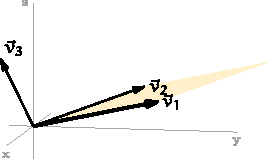
\includegraphics{asy/four_ii_orientation.pdf}}%
                 \only<2->{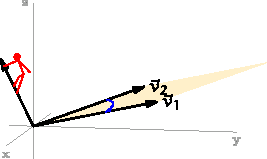
\includegraphics{asy/four_ii_orientation_pos.pdf}}}
\end{equation*}
\pause
Take a $\vec{v}_3$ above that plane.
More precisely, the $\vec{v}_3$ shown is on the side of the plane
with the property that 
a person at the tip of $\vec{v}_3$ 
looking at the arc from $\vec{v}_1$ to~$\vec{v}_2$
sees that arc as counterclockwise.
Any such vector defines a box that is positive-sized.
\begin{equation*}
  \vec{v}_3=\colvec{0 \\ -1 \\ 2}
  \qquad
  \begin{vmat}
    1 &-2 &0 \\
    4 &3 &-1 \\
    1 &1 &2
  \end{vmat}=25
\end{equation*}
\end{frame}
\begin{frame}
This is the \textit{right~hand rule}:~place your right hand's pinky finger
on the spanned plane so that your fingers curl from $\vec{v}_1$ to~$\vec{v}_2$.
Then vectors on the side of the plane with your thumb define
positive-sized boxes. 
\begin{equation*}
  % \vec{v}_1=\colvec{1 \\ 4 \\ 1},\,
  % \vec{v}_2=\colvec{-2 \\ 3 \\ 1},\,
  % \vec{v}_3=\colvec{0 \\ -1 \\ 2}
  % \qquad
  \vcenteredhbox{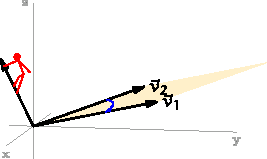
\includegraphics{asy/four_ii_orientation_pos.pdf}}
\end{equation*}
\end{frame}
\begin{frame}
A vector on the plane's other side,
such as $-\vec{v}_3$, will have the same arc from $\vec{v}_1$ to~$\vec{v}_2$
look clockwise and will define a negative-sized box.
\begin{equation*}
  \begin{vmat}
    1 &-2 &0 \\
    4 &3 &1 \\
    1 &1 &-2
  \end{vmat}=-25
\end{equation*}
\only<1-6>{These pictures start above the plane, the perspective of 
the prior slide.}
\only<7->{From below, to a person standing on $-\vec{v}_3$, 
     the arc is clockwise.}
\only<1>{\centergraphic{asy/four_ii_orientation_neg0.pdf}}%
\only<2>{\centergraphic{asy/four_ii_orientation_neg1.pdf}}%
\only<3>{\centergraphic{asy/four_ii_orientation_neg2.pdf}}%
\only<4>{\centergraphic{asy/four_ii_orientation_neg3.pdf}}%
\only<5>{\centergraphic{asy/four_ii_orientation_neg4.pdf}}%
\only<6>{\centergraphic{asy/four_ii_orientation_neg5.pdf}}%
\only<7>{\centergraphic{asy/four_ii_orientation_neg6.pdf}}%
\only<8>{\centergraphic{asy/four_ii_orientation_neg7.pdf}}%
\only<9>{\centergraphic{asy/four_ii_orientation_neg8.pdf}}%
\only<10>{\centergraphic{asy/four_ii_orientation_neg9.pdf}}%
\only<11->{\centergraphic{asy/four_ii_orientation_neg10.pdf}}%
\only<11->{To have it so that when
  you curl your fingers from $\vec{v}_1$ to~$\vec{v}_2$ then
  the vector lies with your thumb, you must use your left hand.}
\end{frame}




\begin{frame}{Determinants are multiplicative}
\th[th:MatChVolByDetMat]%   
\ExecuteMetaData[\detdir det2.tex]{th:MatChVolByDetMat}

\pause
\pf
\ExecuteMetaData[\detdir det2.tex]{pf:MatChVolByDetMat0}

\pause
\ExecuteMetaData[\detdir det2.tex]{pf:MatChVolByDetMat1}
\end{frame}
\begin{frame}
\ExecuteMetaData[\detdir det2.tex]{pf:MatChVolByDetMat2}
\qed
\end{frame}
\begin{frame}
\ex
The transformation $\map{t_{\theta}}{\Re^2}{\Re^2}$ 
that rotates all vectors through a counterclockwise
angle~$\theta$ is represented 
by this matrix.
\begin{equation*}
  T_\theta=
  \rep{t_\theta}{\stdbasis_2,\stdbasis_2}
  =
  \begin{mat}
    \cos\theta  &-\sin\theta \\
    \sin\theta  &cos\theta
  \end{mat}
\end{equation*}
Observe that $t_\theta$ doesn't change the size of any boxes, it just rotates 
the entire box as a rigid whole.
Note that $\deter{T_\theta}=1$.

\pause
\ex The linear transformation $\map{s}{\Re^2}{\Re^2}$
represented with respect to the standard basis by this matrix
\begin{equation*}
  S=
  \begin{mat}
    1 &2 \\
    3 &4
  \end{mat}
\end{equation*}
will, by the theorem, change the size of a box by a factor of $\deter{S}=-2$.
Here is $s$ acting on a typical box. 
\end{frame}
\begin{frame} 
The box defined by the two vectors $\vec{v}_1=\binom{1}{0}$ and
$\vec{v}_2=\binom{1}{1}$ is transformed by~$s$ to the box defined by the 
two vectors $s(\vec{v}_1)=\binom{1}{3}$ and 
$s(\vec{v}_2)=\binom{3}{7}$. 
\begin{center}
  \vcenteredhbox{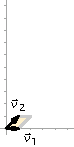
\includegraphics{asy/four_ii_2dtransedsizea.pdf}}
  \qquad$\underrightarrow{s}$\qquad
  \vcenteredhbox{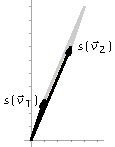
\includegraphics{asy/four_ii_2dtransedsizeb.pdf}}
\end{center}
Note the change in orientation, matching that the determinant is 
negative.

\pause
The two sizes are easy.
\begin{equation*}
  \begin{vmat}
    1 &1 \\ 
    0 &1  
  \end{vmat}
  =1
  \qquad
  \begin{vmat}
    1 &3 \\ 
    3 &7  
  \end{vmat}
  =-2
\end{equation*}
\end{frame}


\begin{frame}{Determinant of the inverse}
\co[co:DeterminantOfInverseIsInverseOfDeterminant]  
\ExecuteMetaData[\detdir det2.tex]{co:DeterminantOfInverseIsInverseOfDeterminant}

\pause
\pf
\ExecuteMetaData[\detdir det2.tex]{pf:DeterminantOfInverseIsInverseOfDeterminant}
\qed

\ex These matrices are inverse.
\begin{equation*}
  \begin{vmat}
    1 &2 \\
    3  &4
  \end{vmat}
  =-2
  \qquad
  \begin{vmat}
    -2 &1 \\
    3/2  &-1/2
  \end{vmat}
  =-1/2
\end{equation*}

\end{frame}




\begin{frame}{Volume}
\df[df:Volume]  
\ExecuteMetaData[\detdir det2.tex]{df:Volume}

\ex 
The box formed by the vectors 
\begin{equation*}
  \sequence{\vec{v}_1,\vec{v}_2}
  =\sequence{\colvec[r]{-1 \\ 1},
             \colvec{1 \\ 1}}
  \hspace*{4em}
  \vcenteredhbox{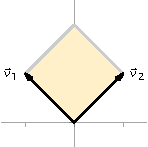
\includegraphics{asy/four_ii_negvolbox.pdf}}
\end{equation*}
gives this determinant
\begin{equation*}
  \begin{vmat}[r]
    -1 &1 \\
     1 &1
  \end{vmat}
  =-2
\end{equation*}
so its volume is~$2$.
\end{frame}




% ..... Four.Topic .....
\section{Cramer's Rule}
%..........
\begin{frame}{Geometric interpretation of linear systems}
\ExecuteMetaData[\detdir cramer.tex]{CramersRuleExample0}
% \begin{center}
%  \includegraphics{\detmpdir ch4.1}
% \end{center}
\ExecuteMetaData[\detdir cramer.tex]{CramersRuleExample1}
\begin{center}
 \includegraphics{\detmpdir ch4.1}
\end{center}
\end{frame}
\begin{frame}
Consider expanding only one side of the parallelogram.
Compare the sizes of these shaded boxes.
\begin{center}
   \includegraphics{\detmpdir ch4.2}
   \hfil
   \includegraphics{\detmpdir ch4.3}
   \hfil
   \includegraphics{\detmpdir ch4.4}
\end{center}
\pause
\ExecuteMetaData[\detdir cramer.tex]{CramersRuleExample3}
(The last equality is by the first condition in the definition of
determinants, applied to columns.)
\end{frame}
\begin{frame}
\ExecuteMetaData[\detdir cramer.tex]{CramersRuleExample4}
\pause
The symmetric argument for the other side gives the other value.
\begin{equation*}
  x_2=
  \frac{
  \begin{vmat}
    1  &6  \\
    3  &8
  \end{vmat}}{
  \begin{vmat}
    1  &2  \\
    3  &1
  \end{vmat}}
  =2
\end{equation*}
\end{frame}


\begin{frame}{Cramer's Rule}
\th  % was: [Cramer's Rule]
Let $A$ be an $\nbyn{n}$ matrix with a nonzero determinant,
let $\vec{b}$ be an $n$-tall column vector,
and consider the linear system $A\vec{x}=\vec{b}$.
For any~$i\in[1,\ldots,n]$ let $B_i$ be the matrix obtained by
substituting $\vec{b}$ for column~$i$ of $A$.
Then the value of the $i$-th unknown is $x_i=\deter{B_i}/\deter{A}$.

% \medskip
% \nearbyexercise{ex:CramerRule} gives the proof.

\medskip
Of course, if the matrix has a zero determinant then the system does not 
have a unique solution.
\end{frame}
\begin{frame}
\ex
This system
\begin{equation*}
  \begin{linsys}{3}
    2x_1 &+ &x_2 &- &x_3 &= &4 \\
     x_1 &+ &3x_2 &  &   &= &2 \\
         &  &x_2 &- &5x_3 &= &0 \\
  \end{linsys}
\end{equation*}
is 
\begin{equation*}
  \begin{mat}[r]
    2 &1 &-1 \\
    1 &3 &0  \\
    0 &1 &-5
  \end{mat}
  \colvec{x_1 \\ x_2 \\ x_3}
  =
  \colvec{4 \\ 2 \\ 0}
\end{equation*}
and
\begin{equation*}
  \deter{A}=
  \begin{vmat}[r]
    2 &1 &-1 \\
    1 &3 &0  \\
    0 &1 &-5
  \end{vmat}
  =-26
  \qquad
  \deter{B_2}=
  \begin{vmat}[r]
    2 &4 &-1 \\
    1 &2 &0  \\
    0 &0 &-5
  \end{vmat}
  =0
\end{equation*}
so $x_2=0/-26=0$.
\end{frame}
\begin{frame}{A caution}
Cramer's Rule is an interesting application of the geometry.
And, it allows us to mentally solve small systems with
simple numbers.
But don't use it for systems having many variables;
taking a determinant of a general large matrix is very slow.   
\end{frame}




%...........................
% \begin{frame}g
% \ExecuteMetaData[../gr3.tex]{GaussJordanReduction}
% \df[def:RedEchForm]
% 
% \end{frame}
\end{document}
